\section{Workflow for the hybrid-solvent CpHMD in CHARMM} 
The hybrid-solvent CpHMD method makes uses of explicit solvent for conformational dynamics and a GB model for propagating protonation states
\cite{Wallace_Shen_2011_J.Chem.TheoryComput.}.
As all MD simulations, CpHMD consists of three stages: system preparation, equilibration, and production.
We will explain each stage using a specific protein as an example. 
To follow along, the tutorial files for soluble proteins can be 
downloaded from our GitLab website \href{https://gitlab.com/shenlab-amber-cphmd/cphmd-tutorial/-/tree/main/hphmd_charmm}{cphmd-tutorial/hphmd\_charmm}
and for transmembrane proteins, 
the tutorial files can be downloaded from \href{https://gitlab.com/shenlab-amber-cphmd/cphmd-tutorial/-/tree/main/memb_hphmd_charmm}{cphmd-tutorial/memb\_hphmd\_charmm}.
We will use the pH replica-exchange protocol \cite{Wallace_Shen_2011_J.Chem.TheoryComput.}
in all the examples.

 %--------------------------------------------- 
\begin{figure*}[htb!]
    \centering
    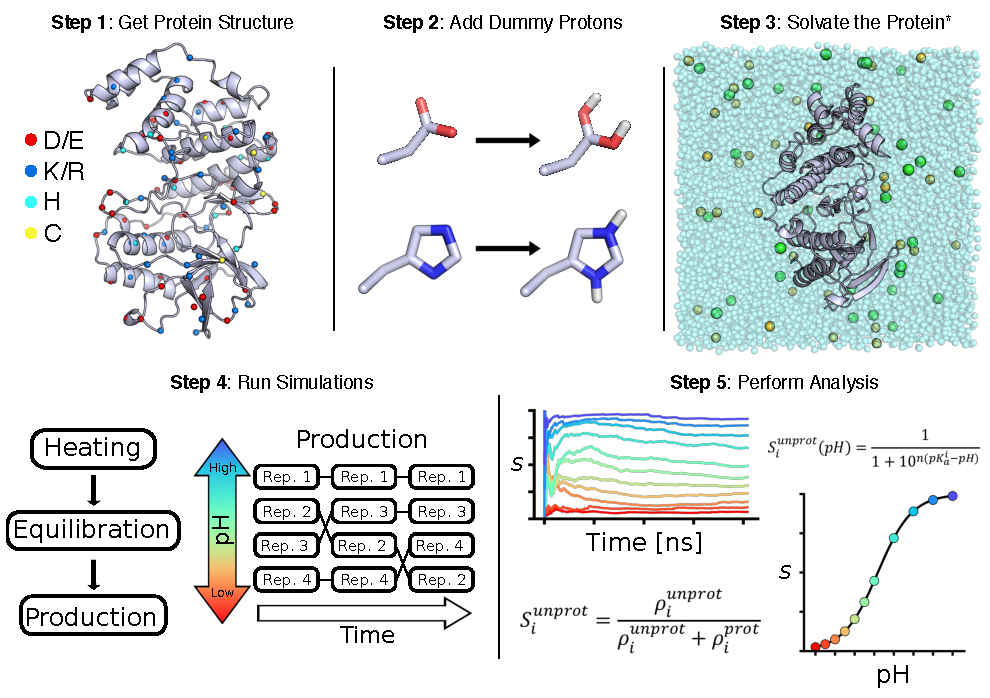
\includegraphics[width=6.6in]{figs/workflow_scheme.pdf}
    \caption{\textbf{Overview of the CpHMD workflow} 
    %Step 5: Add 0 and 1 to the S range.
    %Titration plot, S ==> S_i
    }
    \label{fig:intro}
\end{figure*}
 %--------------------------------------------- 


%------------------------------------------------------------------------------------
\subsection{System Preparation}

To demonstrate CpHMD simulations of 
soluble proteins without retaining the crystal waters,
we use the mini-protein BBL as an example.
The tutorial files for system preparation can be found 
in the directory
\href{https://gitlab.com/shenlab-amber-cphmd/cphmd-tutorial/-/tree/main/hphmd_charmm/bbl_sys_prep}{bbl\_sys\_prep}.

\begin{checklist}{Input files for preparation of a soluble protein}
%\begin{checklist}{Files Produced}
%\textbf{A list of files needed for the equilibration of a soluble protein}
\begin{itemize}
% \item System coordinates (.pdb/.crd)
% \item System topology (.psf)
%%\item Crystal Image Transformations (crystal$\_$image.str)
% \item Periodic boundary conditions (.pbc)
\item step1\_add\_h.inp
\item step2a\_make\_waterbox.inp
\item step2b\_solvate.inp 
\end{itemize}
\end{checklist}

\paragraph{Step 1. Prepare a protein structure with dummy hydrogens.}
First, we retrieve the coordinates of a protein structure
from \href{https://www.rcsb.org/}{Protein Data Bank}\cite{Berman_Bourne_2000_NucleicAcidsRes.},
e.g., BBL (PDB: 1w4h \cite{Ferguson_Fersht_2005_J.Mol.Biol.}).
A homology modeling tool such as SWISS-MODEL\cite{Waterhouse_Schwede_2018_NucleicAcidsRes.} 
can be used to add any missing atomic coordinates.
Next, we convert the PDB file from the standard PDB format to the CHARMM PDB format using the MMTSB tool command \cite{Feig_Brooks_2004_J.Mol.Graph.Model.} \href{http://blue11.bch.msu.edu/mmtsb/convpdb.pl}{convpdb.pl}
or a user supplied script followed by a shell command ``sed'' to
change all histidine residue names to HSP to facilitate titration.

%
\begin{lstlisting}
$ perl convpdb.pl -out charmm22 -segnames
-renumber 1 1w4h.pdb | sed "s/HSD/HSP/g" 
> start.pdb
\end{lstlisting}
%
Here, the output PDB file is formatted for CHARMM (-out charmm22); the segment names are included in the output (-segnames); the residue identification numbers (resid) are renumbered starting at 1; and 
the input file is "1w4h.pdb."
The CHARMM default tautomer for His is HSD.
Changing HSD to HSP indicates to the CpHMD program that histidine is titratable (see later discussion of the parameter file).
Although all resid have been renumbered starting from 1, this does not have to be the case.
Next we add hydrogen atoms to the protein using the HBUILD facility\cite{Brunger_Karplus_1988_Proteins} in CHARMM
\cite{Brooks_Karplus_2009_J.Comput.Chem.}.

To allow titration of Asp and Glu sidechains, we place dummy hydrogens on both carboxylate oxygens.
Note, the dummy atoms do not interact with each other 
and only one is turned on when Asp/Glu is protonated
\cite{Khandogin_Brooks_2005_Biophys.J.}.
The dummy hydrogens are placed in the \textit{syn} position, 
because it is considered
more favorable than the \textit{anti} position
(see discussion in Ref \cite{Khandogin_Brooks_2005_Biophys.J.}).
To prevent the dummy hydrogens from moving to the \textit{anti} position, 
in which case nonnative hydrogen bonds may form
and a neutral dummy may lose the ability to gain charge,
in the CpHMD specific force field parameter file,
the C--O bond rotation energy barrier
is increased from the standard 0.5 to 6.0 kcal/mol
(see discussion in Ref \cite{Khandogin_Brooks_2005_Biophys.J.}).

Following the addition of hydrogens, a brief energy minimization is performed to correct unfavorable positions.
Here 50 steps of steepest descent (SD) and 10 steps of adopted basis Newton-Raphson (ABNR) are used, whereby a harmonic restraint with the force constant of 50 kcal/mol/{\AA}$^2$ is placed on the heavy atoms.
In many experiments, the N- and C-terminal ends of the protein are truncated and require capping. 
For N-terminus we use CH$_3$CO (patch ACE),
and for C-terminus we use NH$_2$ (patch CT2) or NHCH$_3$ (patch CT3).
In special cases, the free ionized forms, NH$_{3}^{+}$ and COO$^-$, 
are used and can be set titratable when CpHMD is turned on. 
The input file 
\href{https://gitlab.com/shenlab-amber-cphmd/cphmd-tutorial/-/tree/main/hphmd_charmm/bbl_sys_prep}
{step1\_add\_h\_prot.inp} is an example of 
how to perform these steps on BBL and can be run with the following command.
%
\begin{lstlisting}[language=bash]
$ charmm -i step1_add_h_prot.inp -o step1.out
\end{lstlisting}
%
The example input also checks for disulfide bonds using a sulfur-to-sulfur distance cutoff of 2.5 {\AA}. 
After running any input file, make sure to visualize the output 
structure to confirm all the dummy hydrogens and additional features are correctly constructed. 

\paragraph{Step 2. Prepare a solvated system}
Now we move to protein solvation by first building a large 
water box of the desired size.
This is done by generating a plane of small cubic water boxes 
along the x- and y-axes, and then stacking the planar water boxes along the z-axis.
CHARMM toppar directory contains the cubic water box made
of pre-equilibrated TIP3P waters.
The size of the large water box is calculated based on the longest
dimension of the protein and a padding space between the protein 
and the edges of the water box.
We recommend having at least $\sim$10 {\AA} padding in x, y, and z directions.
The large cubic water box is then reshaped to a truncated octahedron by removing waters in all eight corners. 
The input file
\href{https://gitlab.com/shenlab-amber-cphmd/cphmd-tutorial/-/tree/main/hphmd_charmm/bbl_sys_prep}
{step2a\_make\_waterbox.inp}
is used to construct the octahedron water box.
%
\begin{lstlisting}[language=bash]
$ charmm -i step2a_make_waterbox.inp -o 
step2_make_waterbox.out
\end{lstlisting}
%
Once the water box is built, the protein is placed at the center and water molecules within 2.8 {\AA} of the protein heavy atoms are deleted.

The solvated system is subject to energy minimization to release unfavorable contacts. 
First, the protein heavy atoms are fixed and the system undergoes energy minimization using SD and ABNR for 50 steps each. 
Next, a five-stage minimization is conducted with the harmonic constants
of 100, 50, 25, 5, and 0 kcal/mol on the protein heavy atoms using 50 steps of SD and 100 steps of ABNR in each stage. 
The input file
\href{https://gitlab.com/shenlab-amber-cphmd/cphmd-tutorial/-/tree/main/hphmd_charmm/bbl_sys_prep}
{step2b\_solvate.inp} can be used.
%
\begin{lstlisting}[language=bash]
$ charmm -i step2b_solvate.inp -o
step2b_solvate.out
\end{lstlisting}
%
Again, always remember to visualize the system and make sure the system has been constructed to your expectations. 

\subsection{System preparation that includes crystal waters}

\begin{checklist}{Required inputs}
%\begin{checklist}{Files Produced}
%\textbf{A list of files needed for the equilibration of a soluble protein}
\begin{itemize}
% \item System coordinates (.pdb/.crd)
% \item System topology (.psf)
%%\item Crystal Image Transformations (crystal$\_$image.str)
% \item Periodic boundary conditions (.pbc)
\item step1a\_add\_h\_prot.inp
\item step1b\_add\_h\_crys\_wat.inp
\item step1c\_merge\_prot\_crys\_wat.inp
\item step2a\_make\_waterbox\_crys\_wat.inp
\item step2b\_solvate\_crys\_wat.inp 
\end{itemize}
\end{checklist}

In some cases the X-ray structure contains water molecules and it is desirable to keep them, e.g., those in the enzyme active site.
A tutorial showing how to set up a system with crystal waters can be
found in the directory \href{https://gitlab.com/shenlab-amber-cphmd/cphmd-tutorial/-/tree/main/hphmd_charmm/crys_wat_system_prep}{crys\_wat\_system\_prep}.
Here we use a small protein, staphylococcus nuclease (SNase), as an example,
as the X-ray structure (PDB ID: 3hzx) contains crystal waters.
To keep the crystal waters, just a few additional steps are needed.
First, move all the water molecules into a separate PDB file and make sure the file is properly formatted with the correct column names and column spacing.
In the tutorial the crystal water coordinates have been exported into the the file
\href{https://gitlab.com/shenlab-amber-cphmd/cphmd-tutorial/-/tree/main/hphmd_charmm/crys_wat_system_prep}
{xwat$\_$original.pdb}; however, this file needs to be reformatted for use in CHARMM. 
The Python script
\href{https://gitlab.com/shenlab-amber-cphmd/cphmd-tutorial/-/tree/main/hphmd_charmm/crys_wat_system_prep}
{mod$\_$xwat.py}
reformats this file to
\href{https://gitlab.com/shenlab-amber-cphmd/cphmd-tutorial/-/tree/main/hphmd_charmm/crys_wat_system_prep}
{xwat$\_$.pdb}.
We should note that most error messages involving the handling of crystal waters are due to the PDB file not being properly formatted. 

Since the crystal waters resolved in a X-ray structure do not contain hydrogen positions, they can be added using the CHARMM input file
\href{https://gitlab.com/shenlab-amber-cphmd/cphmd-tutorial/-/tree/main/hphmd_charmm/crys_wat_system_prep}
{step1b$\_$add$\_$h$\_$crys$\_$wat.inp}.
With hydrogens added to the protein and crystal waters, the two sets of coordinates need to be combined using the CHARMM input file
\href{https://gitlab.com/shenlab-amber-cphmd/cphmd-tutorial/-/tree/main/hphmd_charmm/crys_wat_system_prep}
{step1c$\_$merge$\_$prot$\_$crys$\_$wat.inp}.
The rest of the system preparation is very similar to
that without crystal waters.
The only difference to note is when you solvate the system you can merge the segids of the crystal waters (segid: XWAT) with the bulk water (segid: SOLV) using the following command.
%
\begin{lstlisting}[language=bash]
JOIN XWAT SOLV renumber
RENAME SEGID SOLV sele segid XWAT end
\end{lstlisting}
%
Keep in mind this needs to be done after the deletion of water that overlaps with the protein; otherwise you run the risk of accidentally removing some crystal waters.
An example input file is
\href{https://gitlab.com/shenlab-amber-cphmd/cphmd-tutorial/-/tree/main/hphmd_charmm/crys_wat_system_prep}
{step2b$\_$solvate$\_$crys$\_$wat.inp}.


\subsection{System preparation for transmembrane proteins}

\begin{checklist}{Required inputs}
\begin{itemize}
\item initial$\_$system$\_$prep/step1-5/*.inp
\item initial$\_$system$\_$prep/step6/*.inp
\item final$\_$system$\_$prep/*.inp
\end{itemize}
\end{checklist}
Due to the presence of a lipid bilayer, the preparation of transmembrane proteins for CpHMD simulations requires additional steps.
We divide the preparation into the initial and final stages.
The initial preparation is for fixed-charged equilibration,
whereas the final preparation is for CpHMD simulations.
The related files can be accessed from the directories
\href{https://gitlab.com/shenlab-amber-cphmd/cphmd-tutorial/-/tree/main/memb_hphmd_charmm/initial_system_prep/}{initial\_system\_prep}
and \href{https://gitlab.com/shenlab-amber-cphmd/cphmd-tutorial/-/tree/main/memb_hphmd_charmm/final_system_prep/}{final\_system\_prep}.

To begin the initial system preparation, a solvated protein-membrane system is built.
%we first prepare the protein structure using `step1\_genpsf.inp'.
We start by retrieving the protein structure from the database \href{https://opm.phar.umich.edu/}{OPM} (Orientations of Proteins in Membranes), which properly orients the protein in the lipid bilayer using theoretical calculations and experimental data.\cite{Lomize_Mosberg_2006_Bioinformatics}
Just like for soluble proteins, any missing residues need to be added.
%and then the missing hydrogens can be added.
Here we adopt the standard protonation states, i.e., Asp(-), Glu(-), Cys(0), Lys(+), and Arg(+).
As the solution or model {\pka} of His is 6.54 \cite{Thurlkill_Pace_2006_ProteinSci.}, 
which is within one unit of the physiological pH, special attention needs to be given to its protonation (singly or doubly protonated) and tautomeric state (HSD or HSE) by considering 
the nearby hydrogen bonding and/or salt-bridge interactions. 
% The protonation state of His can be set by changing the residue name in the PDB file and running the script. 
Like soluble proteins, the N- and C-terminal ends may be capped or if necessary the charged forms may be used. 

With the complete protein structure (all heavy atom positions
are in place), we use the script
\href{https://gitlab.com/shenlab-amber-cphmd/cphmd-tutorial/-/tree/main/memb_hphmd_charmm/initial_system_prep/step1-5/step1_genpsf.inp}{step1$\_$genpsf.inp} to build
hydrogen positions followed by a short energy minimization in the GB implicit-solvent model to adjust any energetically
unfavorable hydrogen positions.
Next, we build the rest of the system and equilibrate the
lipid bilayer
following the CHARMM-GUI protocol \cite{Jo_Im_2007_PLoSONE}
for placing the lipids, solvating the system, and adding ions. 
The input files for these steps can be found in the directory \href{https://gitlab.com/shenlab-amber-cphmd/cphmd-tutorial/-/tree/main/memb_hphmd_charmm/initial_system_prep/step1-5}{step1-5}.
Below we will briefly go through the steps.

After the protein structure is prepared, we 
place it at the origin and estimate its 
cross section using the script
\href{https://gitlab.com/shenlab-amber-cphmd/cphmd-tutorial/-/tree/main/memb_hphmd_charmm/initial_system_prep/step1-5/step2.1_orient.inp}{step2.1$\_$orient.inp}. 
The next step is to add water to the pore of the protein 
using the script \href{https://gitlab.com/shenlab-amber-cphmd/cphmd-tutorial/-/tree/main/memb_hphmd_charmm/initial_system_prep/step1-5/step2.2_pwat.inp}{step2.2$\_$pwat.inp}.
To determine the system dimensions the script \href{https://gitlab.com/shenlab-amber-cphmd/cphmd-tutorial/-/tree/main/memb_hphmd_charmm/initial_system_prep/step1-5/step3.1_size.inp}{step3.1$\_$size.inp} is used. 
This script also estimates the lipid type area and the number of lipids required to be placed between the protein boundary and the periodic boundary. 
Approximately 4 to 5 lipids should be placed between the protein and the periodic boundary. 
Additionally, the script calculates the thickness of the water layer above and below the lipid bilayer. 
With the dimensions of the system determined, the lipid heads using big dummy spheres are placed to estimate the positions of the lipids in the bilayer. This is accomplished by \href{https://gitlab.com/shenlab-amber-cphmd/cphmd-tutorial/-/tree/main/memb_hphmd_charmm/initial_system_prep/step1-5/step3.2_packing.inp}{step3.2$\_$packing.inp}.
Next, the dummy spheres are replaced with lipid molecules from a library of randomized conformations using the script \href{https://gitlab.com/shenlab-amber-cphmd/cphmd-tutorial/-/tree/main/memb_hphmd_charmm/initial_system_prep/step1-5/step4.1_lipid.inp}{step4.1$\_$lipid.inp}.
In this example, 1-palmitoyl-2-oleoyl-sn-glycero-3-phosphocholine (POPC) is used, but if other lipids are desired,
the libraries of randomized conformations of lipid molecules can be found in the \href{https://www.charmm-gui.org/?doc=archive&lib=lipid}{CHARMM-GUI Archive - Individual Lipid Molecule Library}.

After the lipid bilayer is built, a rectangular water box is generated using the script \href{https://gitlab.com/shenlab-amber-cphmd/cphmd-tutorial/-/tree/main/memb_hphmd_charmm/initial_system_prep/step1-5/step4.2_waterbox.inp}{step4.2$\_$waterbox.inp}, which solvates the protein/membrane complex.
Next, the number of ions required to achieve the desired salt concentration is calculated, 
and the ions are randomly placed in the slabs of water above and below the membrane. 
In the final step, all of the system components are combined using the script \href{https://gitlab.com/shenlab-amber-cphmd/cphmd-tutorial/-/tree/main/memb_hphmd_charmm/initial_system_prep/step1-5/step5_assembly.inp}{step5$\_$assembly.inp}.

We now relax the assembled protein/membrane system in six stages with gradually reduced harmonic 
restraints using the fixed-charge MD CHARMM-GUI scripts in the directory
\href{https://gitlab.com/shenlab-amber-cphmd/cphmd-tutorial/-/tree/main/memb_hphmd_charmm/initial_system_prep/step6}{step6}.
Following the system relaxation, a much longer (100 ns) simulation in the NPT ensemble is required to fully equilibrate the lipid bilayer.
The protein heavy atoms are harmonically restrained during the simulation.
The progress of the bilayer equilibration is monitored by
the calculation of three properties: surface area per lipid, bilayer thickness, and lipid order parameters \cite{Klauda_Pastor_2010_J.Phys.Chem.B,Huang_Shen_2021_MethodsinMolecularBiology}. 
The system is considered equilibrated when these properties plateau with the simulation time.
Since this can be performed on any scalable or GPU-enabled MD engine using a standard protocol, we leave this step up to the user.

Following the fixed-charge equilibration of the lipid bilayer,
we move to the final system preparation.
Here, we prepare the protein for CpHMD titration by adding dummy hydrogens.
Example input files can be found in the directory \href{https://gitlab.com/shenlab-amber-cphmd/cphmd-tutorial/-/tree/main/memb_hphmd_charmm/final_system_prep}{final\_system\_prep}. 
%to show how the system is prepared for CpHMD equilibration.
The first step to break the final snap shot from the bilayer equilibration into separate components (protein, bilayer, bulk water, pore water, and ions).
We add hydrogens using the script
\href{https://gitlab.com/shenlab-amber-cphmd/cphmd-tutorial/-/tree/main/memb_hphmd_charmm/final_system_prep/step1a_add_h.inp}{step1a$\_$add$\_$h.inp}.
PSF and CRD files are generated for the rest of the system components 
with the following scripts:
\href{https://gitlab.com/shenlab-amber-cphmd/cphmd-tutorial/-/tree/main/memb_hphmd_charmm/final_system_prep/step1b_genpsf_memb.inp}{step1b$\_$genpsf$\_$memb.inp}, 
\href{https://gitlab.com/shenlab-amber-cphmd/cphmd-tutorial/-/tree/main/memb_hphmd_charmm/final_system_prep/step1c_genpsf_water_bulk.inp}{step1c$\_$genpsf$\_$water$\_$bulk.inp}, 
\href{https://gitlab.com/shenlab-amber-cphmd/cphmd-tutorial/-/tree/main/memb_hphmd_charmm/final_system_prep/step1d_genpsf_water_pwat.inp}{step1d$\_$genpsf$\_$water$\_$pwat.inp},
\href{https://gitlab.com/shenlab-amber-cphmd/cphmd-tutorial/-/tree/main/memb_hphmd_charmm/final_system_prep/step1e_genpsf_ion_sod.inp}{step1e$\_$genpsf$\_$ion$\_$sod.inp}, and
\href{https://gitlab.com/shenlab-amber-cphmd/cphmd-tutorial/-/tree/main/memb_hphmd_charmm/final_system_prep/step1f_genpsf_ion_cla.inp}{step1f$\_$genpsf$\_$ion$\_$cla.inp}.
Once all the PSF and CRD files have been made,
the rest of the system can be rebuilt using the script 
\href{https://gitlab.com/shenlab-amber-cphmd/cphmd-tutorial/-/tree/main/memb_hphmd_charmm/final_system_prep/step2_assemble.inp}{step2$\_$assemble.inp}.


%--------------------------------------------------------------------------------
\subsection{Equilibration of soluble proteins}
%--------------------------------------------------------------------------------

\begin{checklist}{Files Required}
\begin{itemize}
\item equil\_hphmd.inp
\end{itemize}
\end{checklist}

Equilibration of soluble proteins for CpHMD is performed at a single pH in several stages. 
An example input for the BBL protein is
\href{https://gitlab.com/shenlab-amber-cphmd/cphmd-tutorial/-/tree/main/hphmd_charmm/bbl_equil_prod}{equil\_hphmd.inp}.
Since CpHMD is turned on during equilibration, titratable residues must be chosen. 
In the example here, Asp, Glu, and His are allowed to titrate because of the pH range used in the production simulation.
The crystal structure pH condition or physiological pH 7.4 can be used.
We specify the physiological ionic strength of 0.15 M and temperature of 298 K.
Before invoking the PHMD module for CpHMD
simulation, we need to call GBSW using the following command.
%
\begin{lstlisting}
GBSW HYBRID SGAMMA 0.005 NANG 50 CONC 0.15 - 
SELE protein END
\end{lstlisting}
%
Here, \textbf{SGAMMA} (default 0.005) is the non-polar surface tension coefficient, \textbf{NANG} (default 50) is the number of angular integration points, and \textbf{CONC} (default 0.15) is the ionic strength in M.
Except for \textbf{CONC}, which the user may change according to the specific problem, the default parameters should be used.

Now we invoke PHMD and set related options using the following command.

\begin{lstlisting}
PHMD PAR 23 WRI 25 PH 7.4 NPRI 5000 PHFRQ 5 
    MASS 10.0 BARR 2.0 BETA 5.0 TEMP 298 LAM -
    SELE RESN ASP .or. RESN GLU .or. RESN HSP end
\end{lstlisting}
%
Here \textbf{PH} is the simulation pH (default 7);
\textbf{NPRI} is the frequency of printing lambda values (5000 means 10 ps);
\textbf{PHFRQ} is the update frequency for the lambda coordinates (default 5);
\textbf{TEMP} is the temperature for $\lambda$ dynamics (default 298);
\textbf{MASS} is the fictitious mass of the $\lambda$ particles (default 10); 
\textbf{BARR} is the quadratic barrier height (default 2.0 and is overwritten by the values specified in the parameter file phmd.inp); 
\textbf{BETA} is the friction coefficient for lambda dynamics (default 5.0); 
\textbf{LAM} tells the PHMD module to output lambda values; and
\textbf{SELE} specifies the types of residues allowed to titrate (default all residues in phmd.inp file). 
Except for PH, NPRI, and SELE options, 
the default parameters should be used.

The length of each stage depends on the system and should be adjusted accordingly.
In the BBL example \href{https://gitlab.com/shenlab-amber-cphmd/cphmd-tutorial/-/tree/main/hphmd_charmm/bbl_equil_prod}{equil\_hphmd.inp},
the heating/equilibration stages were run for 20 ps, 
because the system is very small and stable. 
First, the system is heated in the NVT ensemble, and next
four stages of equilibration are performed in the NPT ensemble with decreasing harmonic restraints on the heavy atom positions, e.g., 5.0, 1.0, 0.1, and 0 kcal/mol/{\AA}$^2$. 
The idea here is to slowly relax the system by removing any high energy contacts and to allow for the initialization of protonation states at the specified pH (e.g., 7).
Note, the equilibration time for the mini-protein BBL
is short, and one can adjust it accordingly for larger proteins.

\subsection{Equilibration of transmembrane proteins}

\begin{checklist}{Required input files}
\begin{itemize}
\item  cphmd$\_$equil/step0.1$\_$equil.inp
\item  cphmd$\_$equil/step0.2$\_$equil.inp
\item  cphmd$\_$equil/step0.3$\_$equil.inp
\end{itemize}
\end{checklist}

Now three short equilibration steps can be performed using CpHMD at a single pH.
Example inputs are in the directory \href{https://gitlab.com/shenlab-amber-cphmd/cphmd-tutorial/-/tree/main/memb_hphmd_charmm/cphmd_equil}{cphmd\_equil}. 
As for a soluble protein, the specified pH should be the pH used in the experiment (e.g., crystal growth, NMR, etc) or physiological pH.
In the first step, the CpHMD simulation is performed 
in the NVT ensemble
with a harmonic force constant of 1.0 kcal/mol/$\mbox{\AA}^2$ for 0.1 ns using
\href{https://gitlab.com/shenlab-amber-cphmd/cphmd-tutorial/-/tree/main/memb_hphmd_charmm/cphmd_equil}{step0.1$\_$equil.inp}.
In the second step, the CpHMD simulation is performed in the NPT ensemble using
\href{https://gitlab.com/shenlab-amber-cphmd/cphmd-tutorial/-/tree/main/memb_hphmd_charmm/cphmd_equil}{step0.2$\_$equil.inp}.
In the third step, the simulation (\href{https://gitlab.com/shenlab-amber-cphmd/cphmd-tutorial/-/tree/main/memb_hphmd_charmm/cphmd_equil}{step0.3$\_$equil.inp}) continues in the NPT ensemble for 0.8 ns with all restraints are removed. 
We note, the membrane-enabled CpHMD simulation makes use of the membrane GBSW model
\cite{Im_Brooks_2003_Biophys.J.}.

\begin{lstlisting}
GBSW HYBRID SGAMMA 0.0 NANG 50 CONC 0.15 - 
     TEMP 310 TMEMB 30 MSW 2.5 -
     RCYLN 15 SELE solu END
\end{lstlisting}
%
The options \textbf{TMEMB}, \textbf{MSM}, and \textbf{RCYLN} are used 
to specify a low dielectric slab in the GBSW model with a high dielectric cylinder centered in the protein.
\textbf{TMEMB} specifies the slab thickness ($\mbox{\AA}$) and should be set to the average difference in the $Z$ positions of the lipid C2 atoms from the top and bottom leaflets. This will vary for different lipid types. 
\textbf{MSM} specifies the half membrane switching length for the dielectric transition between the low-dielectric slab and the bulk solution; 
the default is 2.5 {\AA}.
Finally, \textbf{RCYLN} is the radius of a high dielectric water cylinder placed in the center of the protein; 
it should be set to an appropriate value such that the water cylinder covers the entire protein but does not overlap with lipids as much as possible.
Although no positional restraints are placed on the protein, we recommend using a cylindrical restraint with a harmonic force constant of 0.1 kcal/mol/{\AA}$^{2}$ to prevent the protein from a lateral drift. 
This can be done using the MMFP facility in CHARMM \cite{Brooks_Karplus_2009_J.Comput.Chem.}.

\subsection{Production}

\begin{checklist}{Files Produced}
\begin{itemize}
\item CpHMD Trajectories per pH (.dcd)
\item Lambda Values per pH (.lamb)
\item Replica Exchange Info. per pH (.log)
\item Energy Output per pH (.ene)
\item MD Info. per pH (.out)
\item Restarts per pH (.rst)
\end{itemize}
\end{checklist}

The CpHMD production stage is similar for soluble and transmembrane proteins. The only difference is that the GBSW command includes additional options for the lipid bilayer (see discussion of the equilibration steps) for transmembrane protein simulations.
An example input for the production run of a
soluble protein is
\href{https://gitlab.com/shenlab-amber-cphmd/cphmd-tutorial/-/tree/main/hphmd_charmm/bbl_equil_prod}{prod$\_$hphrex.inp}.
A similar production input for a transmembrane protein is
\href{https://gitlab.com/shenlab-amber-cphmd/cphmd-tutorial/-/tree/main/memb_hphmd_charmm/prod}{prod$\_$hphrex.inp}.
An example job submission file for a HPC cluster is 
\href{https://gitlab.com/shenlab-amber-cphmd/cphmd-tutorial/-/tree/main/memb_hphmd_charmm/prod}{hphrex.qsub}.

To begin the production run one must choose a pH range and number of pH replicas. 
The proper choice of the pH range depends on the research objective.
For example, the pH range of 1.5--6.5 was used in the hybrid-solvent CpHMD study
of the pH-dependent structure function relationship of the endosomal protein BACE1
in which the catalytic aspartyl residues play a central role \cite{Ellis_Shen_2015_J.Am.Chem.Soc.}.
On the other hand, the pH range 4--8 was used in the membrane-enabled hybrid-solvent 
CpHMD study of the pH-dependent conformational activation of the transmembrane M2 channel,
whereby the titration of four histidines modulates the conformation of the channel \cite{Chen_Shen_2016_J.Phys.Chem.Lett.}.
Next, one needs to choose the total number of pH replicas. 
The spacing of the pH conditions needs to be close enough such that sufficient exchange 
probabilities (e.g., at least 20$\%$) are obtained.
To obtain good overlap between potential energy distributions of neighboring replicas
a pH spacing of 0.5 and sometimes even 0.25 is required. 
Other aspects to consider are the number of available CPUs on the HPC and how many CPUs can be 
allocated to each replica. 
Simulations with CHARMM do not scale well past 8 CPUs, so for a job using 16 replicas
we recommend requesting a total of 128 CPUs with 8 CPUs for each replica. 
We recommend making exchange attempts every 1000 MD steps.
A typical pH replica-exchange CpHMD simulation has an average exchange ratio of $\sim$40$\%$, 
but if the exchange ratios are too low, more replicas can be added to fill in the spacing 
between replicas.
To achieve optimum performance in enhanced sampling, several replicas should move 
across all pH conditions.

To use pH-based replica exchange in CHARMM, one can use the 
\href{https://hpc.nih.gov/apps/charmm/c39b2html/repdstr.html}{REPD} module.
%
\begin{lstlisting}
REPD NREP 8 PHMD EXLM FREQ 5000 UNIT 17
\end{lstlisting}
%
Here, the \textbf{REPD} command initiates replica exchange, and \textbf{NREP} states the number of replicas to use
(in this case 8). 
\textbf{PHMD EXLM} states this is a special type of Hamiltonian exchange (i.e., pH-based) and allows for the exchange of pH conditions of two adjacent replicas.
\textbf{FREQ} states the frequency of an exchange attempt. 

Then, to run several replicas in parallel, CHARMM reads in a rep.cmd file for each pH replica 
with the syntax, rep.cmd$\_$0, rep.cmd$\_$1, to rep.cmd$\_$(NREPS), using the following 
command in the input file.
%
\begin{lstlisting}[language=bash]
$ stream rep.cmd
\end{lstlisting}
% 
Notice this command lacks the '$\_0$' portion of the name.
In each of the rep.cmd file you will have the command that states the pH environment of the replica.
%
\begin{lstlisting}
PHMD RESPH OLDPH @crysph NEWPH @ph PKATEMP @temp
\end{lstlisting}
%
Here \textbf{OLDPH} is the pH used in the equilibration and \textbf{NEWPH} is the pH of the replica.
Finally, \textbf{PKATEMP} should be set to the same temperature of the simulation. 
The rest of the replica exchange set up follows a standard MD run in CHARMM.
Production run inputs for BBL (prod$\_$hphrex.inp and rep.cmd) can be used to run one 2 ns stage of pH-Replica Exchange CpHMD.

\subsection{General settings for MD and CpHMD in CHARMM}
% CHARMM Specific
% Things to Include: 
%   -) FFs
%   -) Thermostats
%   -) Baristas
%   -) Cutoffs
%   -) ect...

For all simulations the protein 
is represented by CHARMM22/CMAP force field.\cite{MacKerell_Karplus_1998_J.Phys.Chem.B,MacKerell_Brooks_2004_J.Am.Chem.Soc.}
Note, the current CpHMD methods are not compatible with the CHARMM36 protein force field.
For solvent the CHARMM modified TIP3P water model is used.
For ions or lipid molecules the CHARMM36 force fields are used \cite{Klauda_Pastor_2010_J.Phys.Chem.B}.
The van der Waals energies are calculated with a switching function from 10 to 12 {\AA} and  a cutoff at 14 {\AA}. 
All simulations are conducted under periodic boundary conditions. 
The PME method \cite{Darden_Pedersen_1993_J.Chem.Phys.} is used to calculate the long-range electrostatic energies and forces with a real space calculation cutoff of 12 {\AA} and 1 {\AA} grid spacing, and a 6th-order spline interpolation. 
The non-bond neighbor list is updated heuristically. 
Additionally, the SHAKE \cite{Ryckaert_Berendsen_1977_J.Comput.Phys.} algorithm is used to constrain all bonds involving hydrogens to allow for a 2-fs time step. 
For NPT simulations, the temperature is maintained with the N\'{o}se-Hoover thermostat \cite{Nose_Nose_1984_Mol.Phys.,Hoover_Hoover_1985_Phys.Rev.Aa}.
The pressure is maintained with the Langevin piston pressure-coupling algorithm \cite{Feller_Brooks_1995_J.Chem.Phys.}.
For the CpHMD simulations, the default GBSW radii \cite{Nina_Roux_1997_J.Phys.Chem.B,Chen_Brooks_2006_J.Am.Chem.Soc.} are used for the protein.
For small molecules, the generic atomic radii in the GBSW file may be used upon user verification. 
A CpHMD parameter file phmd.inp contains
the model reference {\pka} values and the parameters in the titration potential of mean force for Asp, Glu, His, Cys, and Lys. 
Parameters for additional titratable groups
can be obtained by following the steps discussed in section Parameterization.
% As shown in the example inputs the titration ($\lambda$) and tautomer ($\chi$) should be updated every 5 MD steps, allowing for water and lipid relaxation.\cite{Wallace_Shen_2011_J.Chem.TheoryComput.}
% A friction coefficient of 5 ps$^{-1}$ should be used for Langevin dynamics and the mass of the titration coordinate ($\lambda$ and $\chi$) should be 10 atomic mass units. https://www.overleaf.com/project/60d33785a3cd6c24e62c6d32